\section{Classification}
Our primary objective is separating experimental data into two possible categories.
Supervised learning typically leverages large amounts of labeled data to learn
representations of the classes present in the inputs. A challenge in Physics is that
experiments generate enormous amounts of data, but it is not labeled. Hand-labeling
data is time-consuming and cost-ineffective. A possible solution to this challenge
is to train models on simulated data. The idea being that simulated and experimental
data are similar enough that the learned patterns from simulated data are, to some degree,
transferrable to experimental data.
The simulated data contains two classes of events - a single electron and a double electron.
\subsection{Simulated data}
In table \ref{tab:classification-simulated-f1} the performance of each model trained is reported
as the f1-score. The model architecture for each model is described in (ref appendix).
... including a state of the art pretrained network (\cite{}VGG HERE) applied to the data using
the approach described in \ref{section:chapter-pretrained}.
\begin{table}
\centering
\caption{
Mean F1-scores for classification of simulated data using multiple models. 
Error estimates are the standard deviation in results from k-fold cross-validation 
with $K=5$ folds.
}
\label{tab:classification-simulated-f1}
\begin{tabular}{llll}
\toprule
                                           Logistic &                                               Dense &                                       Convolutional &                                    Pretrained VGG16 \\
\midrule
 $\underset{\num{+- 7.727e-03 }  }{\num{ 0.734 } }$ &  $\underset{\num{+- 1.329e-02 }  }{\num{ 0.907 } }$ &  $\underset{\num{+- 6.286e-03 }  }{\num{ 0.959 } }$ &  $\underset{\num{+- 1.591e-02 }  }{\num{ 0.894 } }$ \\
\bottomrule
\end{tabular}
\end{table}

To give a broader picture of the performance we also include the confusion matrix values in
table \ref{tab:classification-simulated-confmat}. Similar f1-scores may still show differences
in either of the confusion matrix values.
\begin{table}
\centering
\caption{
Mean confusion matrix values for classification of simulated data using multiple models. 
Error estimates are the standard deviation in results from k-fold cross-validation with $K=5$ folds.
}
\label{tab:classification-simulated-confmat}
\begin{tabular}{lllll}
\toprule
{} &                                                     TN &                                                     FP &                                                     FN &                                                     TP \\
\midrule
Logistic         &  $\underset{\num{+- 1.546e+04 }  }{\num{ 1.28e+05 } }$ &  $\underset{\num{+- 1.546e+04 }  }{\num{ 6.16e+04 } }$ &  $\underset{\num{+- 1.118e+04 }  }{\num{ 4.39e+04 } }$ &  $\underset{\num{+- 1.118e+04 }  }{\num{ 1.46e+05 } }$ \\
Dense            &  $\underset{\num{+- 1.125e+04 }  }{\num{ 1.72e+05 } }$ &  $\underset{\num{+- 1.125e+04 }  }{\num{ 1.85e+04 } }$ &  $\underset{\num{+- 5.205e+03 }  }{\num{ 1.73e+04 } }$ &  $\underset{\num{+- 5.205e+03 }  }{\num{ 1.73e+05 } }$ \\
Convolutional    &  $\underset{\num{+- 7.287e+02 }  }{\num{ 1.89e+05 } }$ &  $\underset{\num{+- 7.290e+02 }  }{\num{ 1.39e+03 } }$ &  $\underset{\num{+- 2.692e+03 }  }{\num{ 1.37e+04 } }$ &  $\underset{\num{+- 2.692e+03 }  }{\num{ 1.76e+05 } }$ \\
Pretrained VGG16 &  $\underset{\num{+- 9.079e+03 }  }{\num{ 1.79e+05 } }$ &  $\underset{\num{+- 9.080e+03 }  }{\num{ 1.15e+04 } }$ &  $\underset{\num{+- 9.409e+03 }  }{\num{ 2.71e+04 } }$ &  $\underset{\num{+- 9.408e+03 }  }{\num{ 1.63e+05 } }$ \\
\bottomrule
\end{tabular}
\end{table}

\ref{tab:classification-simulated-confmat}.
\begin{figure}
\centering
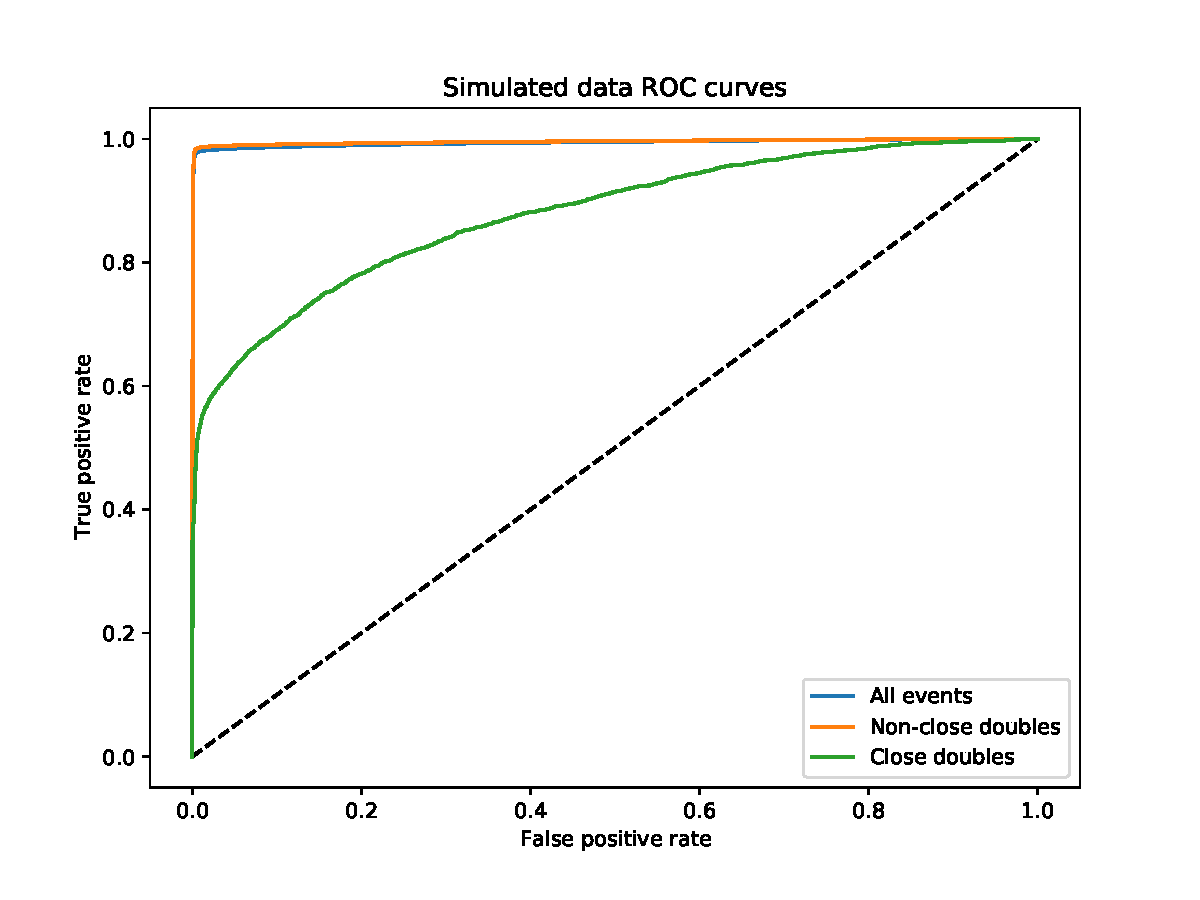
\includegraphics[width=0.8 \textwidth]{chapters/results/figures/roc_simulated.pdf}
\caption[Titletext]{generic text}\label{fig:roc_simulated}
\end{figure}
\subsection{Regression}

\begin{itemize}
  \item ? - Linear approach?
  \item ? - Dense network
  \item ? - CNN
\end{itemize}
\subsection{Experimental data}
\section{Regression}
\subsection{Position}
\subsection{Energy}
\subsection{Position}
\subsection{Energy}
